\documentclass[11pt,letterpaper]{article}
\usepackage[lmargin=1in,rmargin=1in,tmargin=1in,bmargin=1in]{geometry}
\usepackage{../style/homework}
\usepackage{../style/commands}
\setbool{quotetype}{false} % True: Side; False: Under
\setbool{hideans}{false} % Student: True; Instructor: False

% -------------------
% Content
% -------------------
\begin{document}

\homework{11: Due 12/09}{Earth is amazing! There are these things called farms. They put seeds in the ground, pour water on them, and they grow into food, like pizzas!}{Captain, Wall-E}

% Problem 1
\problem{10} The probabilities of several events in a finite probability space are given below:
	\[
	\begin{aligned}
	P(A)&= 0.45 & P(A \text{ and } B)&= 0.11 \\
	P(B)&= 0.21 & P(A \text{ and } C)&= 0.81 \\
	P(C)&= 0.73 & P(B \text{ and } C)&= 0.00 \\
	P(D)&= 0.55 & P(B \text{ or } D)&= 0.71
	\end{aligned}
	\] 
\begin{enumerate}[(a)]
\item Find $P(A \text{ or } B)$. 
\item Assuming $A$ and $D$ are independent events, find $P(A \text{ and } D)$.
\item Find $P(A \;|\; B)$.
\item Find $P(B \text{ and } D)$. 
\item Are $C$ and $D$ disjoint? Explain.
\item Are $A$ and $C$ independent? Explain.
\item Are $B$ and $C$ independent? Explain.
\end{enumerate} \pspace

\sol
\begin{enumerate}[(a)]
\item 
	\[
	P(A \text{ or }B)= P(A) + P(B) - P(A \text{ and }B)= 0.45 + 0.21 - 0.11= 0.55
	\]

\item 
	\[
	P(A \text{ and }D)= P(A) \cdot P(D)= 0.45 \cdot 0.55= 0.2475
	\]

\item 
	\[
	P(A \;|\; B)= \dfrac{P(A \text{ and }B)}{P(B)}= \dfrac{0.11}{0.21}= 0.5238
	\]

\item 
	\[
	\begin{gathered}
	P(B \text{ or }D)= P(B) + P(D) - P(B \text{ and }D) \\
	0.71= 0.21 + 0.55 - P(B \text{ and }D) \\
	P(B \text{ and }D)= 0.76 - 0.71 \\
	P(B \text{ and }D)= 0.05
	\end{gathered}
	\]

\item If $C$ and $D$ were disjoint, then $P(C \text{ or }D)= P(C) + P(D)= 0.73 + 0.55= 1.28 > 1$, which is impossible. Therefore, $C$ and $D$ cannot be disjoint. 

\item If $A$ and $C$ were independent, then $P(A \text{ and }C)= P(A) \cdot P(C)$. But $P(A \text{ and }C)= 0.81$ while $P(A) \cdot P(C)= 0.45 \cdot 0.73= 0.3285$. Therefore, $A$ and $C$ are not independent. 

\item We see that $P(B \text{ and }C)= 0.00$. Therefore, $B$ and $C$ are disjoint. But then $B$ and $C$ cannot be independent because disjoint events are never independent. 
\end{enumerate}





\newpage





% Problem 2
\problem{10} At a financial analysis firm with 66 employees, 37 employees perform algorithmic trading as part of their job, 16 perform audits, and 3 perform both. 
        \begin{enumerate}[(a)]
        \item Find the probability that a randomly selected employees performs algorithmic trading or audits. 
        \item Find the probability that a randomly selected employees performs neither algorithmic trading or nor audits. 
        \item Find the probability that a randomly selected employees only performs audits as part of their job.
        \item Find the probability that an employee that performs audits also performs algorithmic trading as part of their job. 
        \item Find the probability that a randomly selected employee performs both audits and algorithmic trading as part of their job. 
        \end{enumerate} 

\sol
\begin{enumerate}[(a)]
\item 
	\[
	P(\text{Algo. or Audit})= \dfrac{34 + 3 + 13}{66}= \dfrac{50}{66} \approx 0.7576
	\]
		\begin{center} OR \end{center}
	\[
	P(\text{Algo. or Audit})= P(\text{Algo.}) + P(\text{Audit}) - P(\text{Algo. and Audit})= \dfrac{37}{66} + \dfrac{16}{66} - \dfrac{3}{66}= \dfrac{50}{66} \approx 0.7576
	\] 

\item 
	\[
	P(\text{neither Algo. nor Audit})= \dfrac{16}{66} \approx 0.2424
	\] 

\item 
	\[
	P(\text{only Audit})= \dfrac{13}{66} \approx 0.1970
	\] 

\item 
	\[
	P(\text{Algo.} \;|\; \text{Audits})= \dfrac{P(\text{Algo. and Audit})}{P(\text{Audits})}= \dfrac{3/66}{16/66}= \dfrac{3}{16} \approx 0.1875
	\]

\item 
	\[
	P(\text{Algo. and Audit})= \dfrac{3}{66} \approx 0.0455
	\]
\end{enumerate}

	\[
	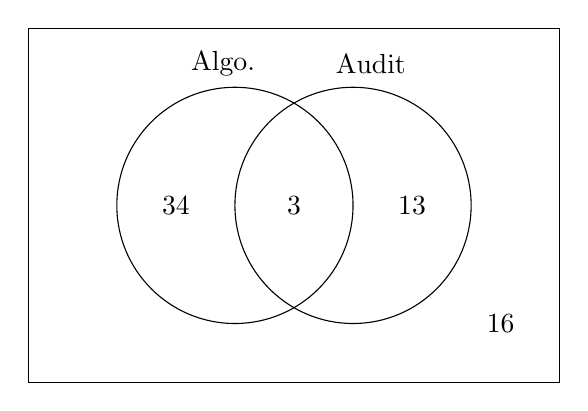
\begin{tikzpicture}[scale=0.75]
	\draw (0,0) rectangle (9,6);
	\draw (3.5,3) circle (2);
	\draw (5.5,3) circle (2);
	
	\node at (3.3,5.4) {Algo.};
	\node at (5.8,5.4) {Audit}; 
	
	\node at (2.5,3) {34};
	\node at (4.5,3) {3};
	\node at (6.5,3) {13};
	\node at (8,1) {16};
	\end{tikzpicture}
	\]





\newpage





% Problem 3
\problem{10} A construction company places bids on various construction projects. The company underbids 30\% of the time. If they underbid, they get the job 80\% of the time. If they do not underbid, they fail to get the job 90\% of the time. 
	\begin{enumerate}[(a)]
	\item Find the probability that they underbid and get the job.
	\item Find the probability that they get the job, if they make a bid. 
	\item Find the probability that they get the job or underbid. 
	\item Find probability that they did not underbid, if they got the job. 
	\end{enumerate} \pspace

\sol
\begin{enumerate}[(a)]
\item 
	\[
	P(\text{Under and Get})= 0.24 
	\] \pspace

\item 
	\[
	P(\text{Get})= 0.24 + 0.07= 0.31
	\] \pspace

\item 
	\[
	P(\text{Get or Underbid})= 0.24 + 0.06 + 0.07= 0.37
	\]
		\begin{center} OR \end{center}
	\[
	P(\text{Get or Underbid})= P(\text{Get}) + P(\text{Under}) - P(\text{Get and Under})= (0.24 + 0.07) + (0.24 + 0.06) - 0.24= 0.37
	\] \pspace

\item 
	\[
	P(\text{Not Under} \;|\; \text{Got})= P(\text{Over} \;|\; \text{Got})= \dfrac{P(\text{Over and Got})}{P(\text{Got})}= \dfrac{0.07}{0.24 + 0.07}= \dfrac{0.07}{0.31}= 0.2258
	\]
\end{enumerate} \pspace

		\[
		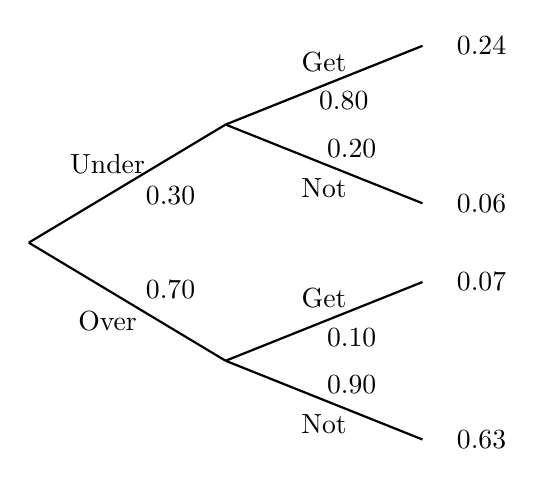
\begin{tikzpicture}[scale= 1.0]
		\def\FirstUpLabel{Under}
		\def\FirstDownLabel{Over}
		\def\SecondUpLabel{Get}
		\def\SecondDownLabel{Not}
		\def\Up{$0.30$}
		\def\Down{$0.70$}
		\def\UpUp{$0.80$}
		\def\UpDown{$0.20$}
		\def\DownUp{$0.10$}
		\def\DownDown{$0.90$}
		\def\first{$0.24$}
		\def\second{$0.06$}
		\def\third{$0.07$}
		\def\fourth{$0.63$}
		
		\node at (1,1) {\FirstUpLabel};	
		\node at (1,-1) {\FirstDownLabel};	
		\node at (1.8,0.6) {\Up};
		\node at (1.8,-0.6) {\Down};
		\draw[thick] (0,0) -- (2.5,1.5);
		\draw[thick] (0,0) -- (2.5,-1.5);
		
		\node at (3.75,2.3) {\SecondUpLabel};
		\node at (3.75,0.7) {\SecondDownLabel};
		\node at (4,1.8) {\UpUp};
		\node at (4.1,1.2) {\UpDown};
		\node at (5.75,2.5) {\first};
		\node at (5.75,0.5) {\second};
		\draw[thick] (2.5,1.5) -- (5,2.5);
		\draw[thick] (2.5,1.5) -- (5,0.5);

		\node at (3.75,-0.7) {\SecondUpLabel};
		\node at (3.75,-2.3) {\SecondDownLabel};
		\node at (4.1,-1.2) {\DownUp};
		\node at (4.1,-1.8) {\DownDown};
		\node at (5.75,-0.5) {\third};	
		\node at (5.75,-2.5) {\fourth};	
		\draw[thick] (2.5,-1.5) -- (5,-0.5);
		\draw[thick] (2.5,-1.5) -- (5,-2.5);
		\end{tikzpicture}
		\]





\newpage





% Problem 4
\problem{10} Suppose you play a game where you roll a tetrahedral die with sides labeled one through four. The probabilities for which are (partially) given below. If you roll a four, you must pay \$3; if you roll a two or three, you win nothing; if you roll a one, you win \$20. 
	\begin{table}[!ht]
	\centering 
	\begin{tabular}{|c||c|c|c|c|} \hline 
	$n$ & $1$ & $2$ & $3$ & $4$ \\ \hline 
	$P(n)$ & $\dfrac{1\rule{0pt}{2.9ex}}{10\rule[-1.3ex]{0pt}{0pt}}$ & $\dfrac{2}{10}$ & $\mathit{\dfrac{2}{10}}$ & $\dfrac{5}{10}$ \\ \hline 
	\end{tabular}
	\end{table}

\begin{enumerate}[(a)]
\item Find $P(3)$. 
\item Find the probability that if you roll the die twice, you win both times. 
\item Find the average amount you win per game. 
\item Should you play this game? Explain.
\item Suppose you had to pay \$2 each time you wanted to play this game. How does this affect the answer from (d)? Explain. 
\end{enumerate} \pspace

\sol
\begin{enumerate}[(a)]
\item 
	\[
	1 - \left( \dfrac{1}{10} + \dfrac{2}{10} + \dfrac{5}{10} \right)= 1 - \dfrac{8}{10}= \dfrac{2}{10}
	\]

\item 
	\[
	P(\text{win and win})= P(\text{win}) \cdot P(\text{win})= \dfrac{1}{10} \cdot \dfrac{1}{10}= \dfrac{1}{100}
	\]

\item 
	\[
	EX= \sum X P(X)= 20 \cdot \dfrac{1}{10} + 0 \cdot \dfrac{2}{10} + 0 \cdot \dfrac{2}{10}  - 3 \cdot \dfrac{5}{10}= \dfrac{5}{10}= \dfrac{1}{2}= \$0.50 
	\]

\item Yes. In the long run, the expected value, i.e. the average amount you win per game is \$0.50, which is positive. Therefore in the long run, on average, you are making money each time you play the game. For instance, if one played this game 200 times, one would expect that, on average, the player would then be up $200 \cdot 0.50= \$100$. 

\item You would no longer want to play this game. From (d), you are only winning an average of \$0.50 per game, while you are paying \$2 to play the game. So on average, you are losing \$1.50 per game. We can confirm this with a direct calculation (by factoring in the \$2 paid in the total winnings per roll): 
	\[
	EX= \sum X P(X)= 18 \cdot \dfrac{1}{10} - 2 \cdot \dfrac{2}{10} - 2 \cdot \dfrac{2}{10}  - 5 \cdot \dfrac{5}{10}= -\dfrac{15}{10}= -\$1.50
	\]
\end{enumerate}


\end{document}